\documentclass[11pt]{article}
\usepackage{fontspec}
\usepackage[a4paper,margin=2.3cm]{geometry}
\usepackage{graphicx}
\usepackage{booktabs}
\usepackage{array}
\usepackage{xcolor}
\usepackage{float}
\usepackage{fancyvrb}
\usepackage[hidelinks]{hyperref}

\setmainfont{Helvetica Neue}
\setmonofont{Menlo}
\renewcommand{\arraystretch}{1.25}

\title{\textbf{Athena TTS — Báo cáo similarity}\\[2pt]
\large Engine nào clone giống ``giọng gốc'' nhất?}
\author{}
\date{15/06/2026}

\begin{document}
\maketitle
\vspace{-1.5em}

\section*{1. Mục tiêu}
Dùng \textbf{một kịch bản mới} (khác lần trước), chạy lại qua cả 5 engine với
\textbf{cùng setup} và \textbf{cùng file giọng mẫu} \texttt{refs/speaker.wav} (11s),
rồi đo xem giọng tạo ra của engine nào \textit{giống giọng gốc} nhất. Tất cả chạy CPU
(Apple M4 Pro). Riêng Kokoro không nhân bản giọng (dùng giọng cài sẵn) nên là mốc tham chiếu.

\section*{2. Kịch bản mới được test}
\begin{Verbatim}[frame=single,fontsize=\small,rulecolor=\color{gray}]
The morning train arrived exactly on time today.
She carefully placed the old letters back into the wooden box.
Could you please tell me how to get to the central library?
Numbers like seven, nineteen, and forty-two appear quite often.
Honestly, I did not expect the final results to be this good.
Thank you for listening, and I hope you have a wonderful day.
\end{Verbatim}

\section*{3. Cách đo}
Trích \textit{speaker embedding} (vector đặc trưng giọng) bằng \textbf{Resemblyzer}
(d-vector GE2E), rồi tính \textbf{cosine similarity} giữa output của mỗi engine và
giọng gốc. Càng gần 1.0 càng giống. \par
\textbf{Trần (ceiling) = 0.983}: độ giống giữa hai clip khác nhau của \emph{cùng một người}
(\texttt{speaker.wav} vs \texttt{speaker\_full.wav}) — mức tối đa mà bản clone hoàn hảo có thể đạt.

\section*{4. Kết quả}
\begin{table}[H]\centering
\begin{tabular}{c >{\bfseries}l r r l}
\toprule
\# & Engine & Cosine & \% so với trần & Ghi chú \\
\midrule
1 & F5-TTS     & 0.969 & 99\% & Giống giọng gốc nhất \\
2 & IndexTTS2  & 0.966 & 98\% & Sát nút, cân bằng tốt \\
3 & Chatterbox & 0.953 & 97\% & Clone tốt \\
4 & StyleTTS2  & 0.923 & 94\% & Hơi ``diễn giải'' lại giọng \\
\midrule
-- & Kokoro    & 0.832 & --   & Giọng cài sẵn, không clone (baseline) \\
\bottomrule
\end{tabular}
\end{table}

\begin{figure}[H]\centering
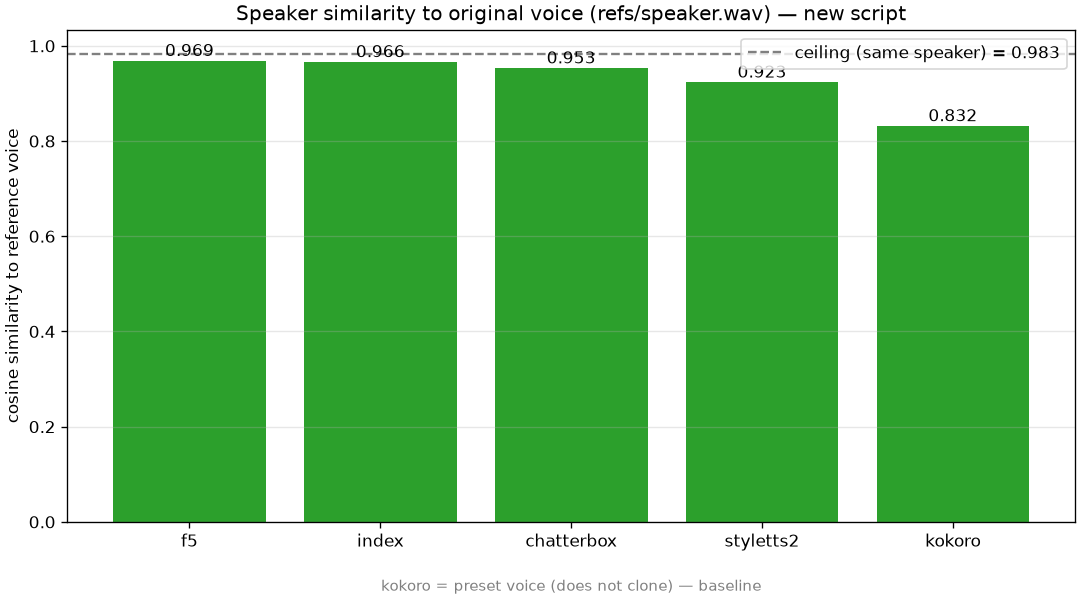
\includegraphics[width=0.92\linewidth]{similarity_chart.png}
\caption{Độ giống giọng gốc của từng engine (đường gạch = trần 0.983).}
\end{figure}

\section*{5. Phát hiện chính: giống giọng $\neq$ tự nhiên}
F5-TTS \textbf{giống giọng gốc nhất} nhưng lại \textbf{kém tự nhiên nhất} (xem báo cáo trước):
kiểu in-context của nó copy timbre của mẫu rất sát (copy cả nét kém ổn định) nên khớp
\emph{danh tính} tốt, nhưng nghe ``máy'' hơn. Ngược lại StyleTTS2 nghe tự nhiên nhất nhưng
giống gốc ít hơn một chút. \textbf{IndexTTS2 cân bằng tốt nhất} — nằm ở góc trên-phải.

\begin{figure}[H]\centering
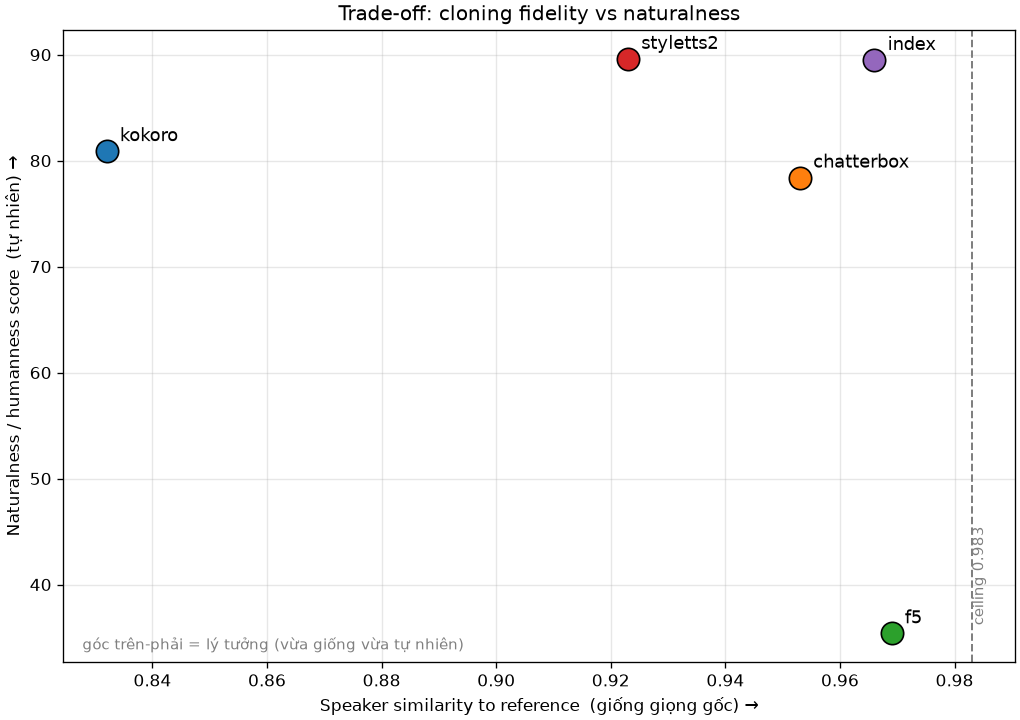
\includegraphics[width=0.82\linewidth]{tradeoff_scatter.png}
\caption{Đánh đổi giữa độ giống giọng (trục ngang) và độ tự nhiên (trục dọc).
Góc trên-phải là lý tưởng: IndexTTS2 gần đó nhất.}
\end{figure}

\begin{figure}[H]\centering
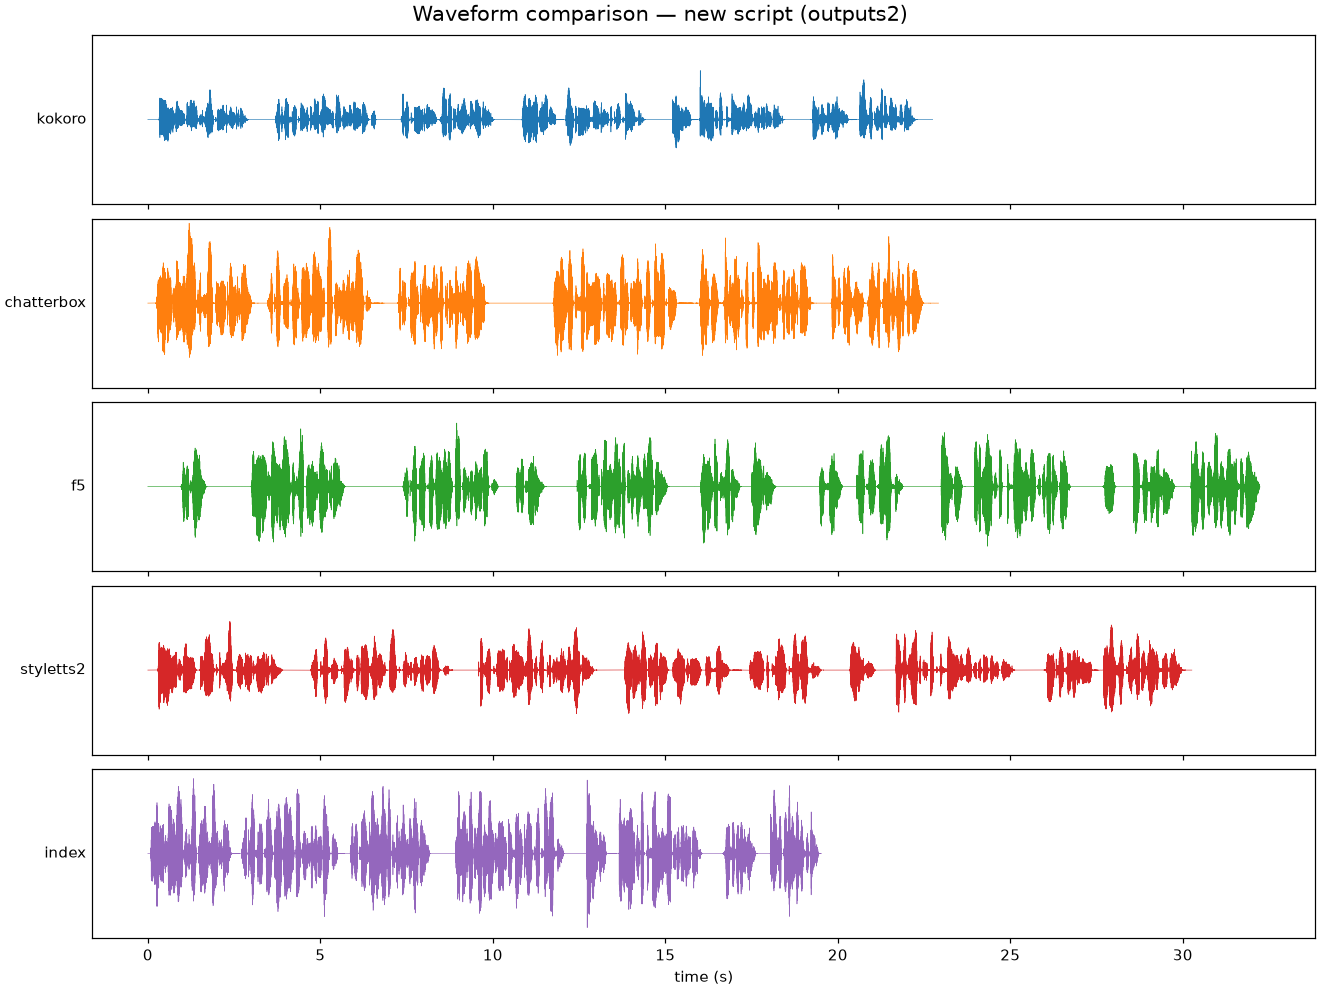
\includegraphics[width=\linewidth]{compare_waveforms2.png}
\caption{Biểu đồ sóng của 5 engine trên kịch bản mới.}
\end{figure}

\begin{figure}[H]\centering
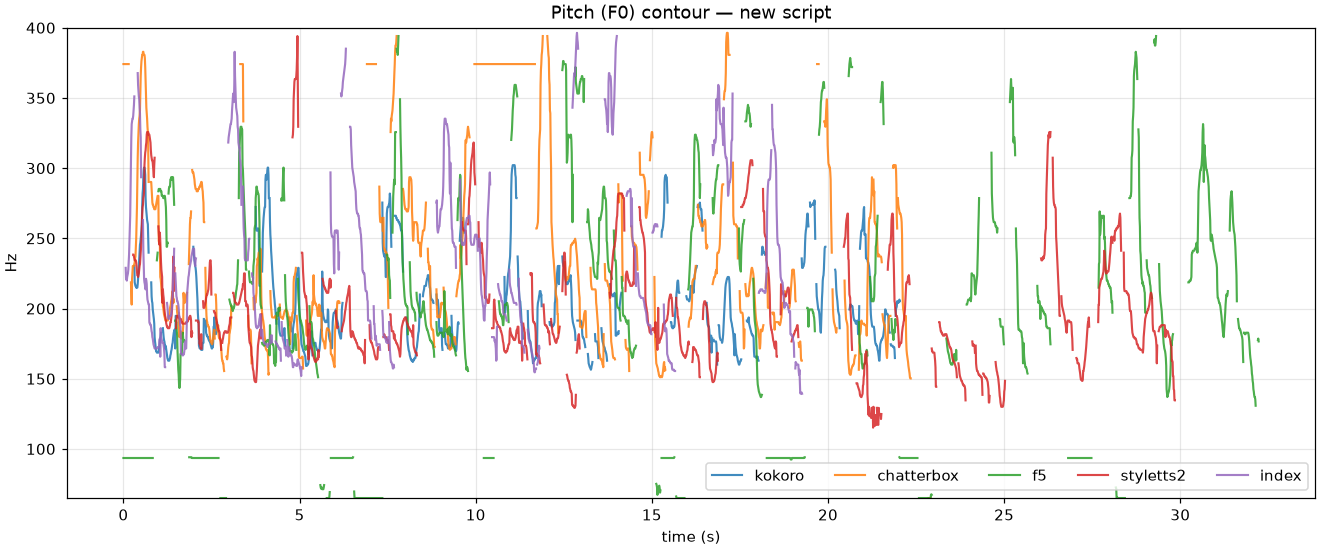
\includegraphics[width=\linewidth]{compare_pitch2.png}
\caption{Đường cao độ (F0) trên kịch bản mới.}
\end{figure}

\section*{6. Kết luận \& gợi ý chọn}
\begin{itemize}\setlength\itemsep{2pt}
\item Cần \textbf{giống giọng gốc nhất} $\rightarrow$ \textbf{F5-TTS} (99\% trần).
\item Cần \textbf{cân bằng giống + tự nhiên + nhanh hơn} $\rightarrow$ \textbf{IndexTTS2} (98\%, hạng 2 về tự nhiên).
\item Cần \textbf{tự nhiên nhất}, chấp nhận giống ít hơn chút $\rightarrow$ \textbf{StyleTTS2}.
\item Cả 4 engine clone đều đạt 0.92--0.97 (rất cao) — chênh lệch nhỏ.
\item Kokoro (0.83) không clone, chỉ hợp khi không cần giữ giọng gốc.
\end{itemize}
\textit{Lưu ý:} cosine similarity là thước đo khách quan tốt cho ``danh tính giọng'',
nhưng vẫn nên nghe trực tiếp để xác nhận cảm nhận cuối cùng.

\end{document}
